\chapter{Algorithm}\label{cp:algo}

This chapter explains the general principles behind the algorithm and separates the logic from the implementation, which will be discussed in a separate chapter, \nameref{cp:sw}. 

- show whole raw dataset and explain where Preprocessing, Deflation and OMWE happens.


\section{Preprocessing}
Only the deflating filtered data is processed by the core algorithm part. The preprocessing part filters the data and detects if the pressure is high enough to start the deflation process. 

\subsection{Filtering}
Show filters
%All data is filtered. 
\subsection{Inflation Detection}
Currently implemented only if is high enough. For future: include deflation rate calculation (and possible feedback / cancellation of measurement)
\section{Deflation}
explain graph

\begin{figure}[ht]
\centering
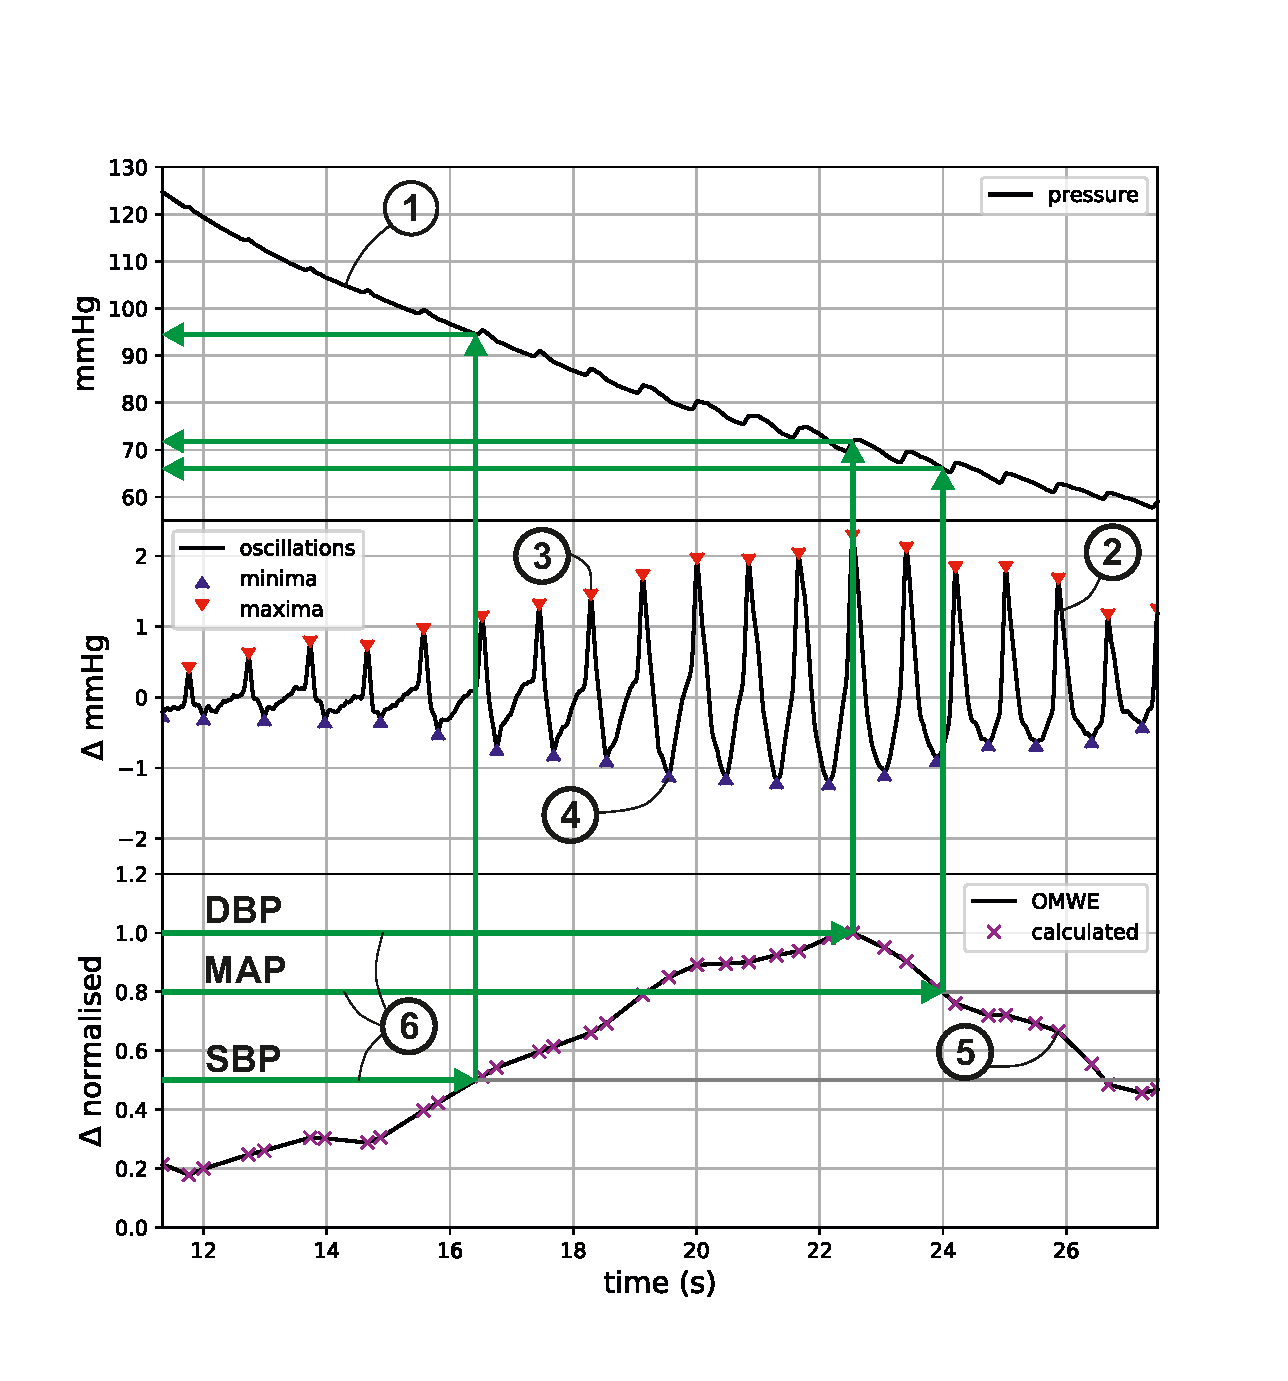
\includegraphics[width=\textwidth]{figures/algorithm_example_annotated.pdf}
\caption{Algo explanation.}
\label{fig:CD}
\end{figure}

\subsection{Extrema Detection}
minima
maxima

\subsection{Heart Rate Detection}
calculation of momentary heart beat from last two maxima



\section{Oscillometric Wave Envelope}
Interpolation between extrema to calculate Oscillometric Wave Envelope (OMWE).

\subsection{Determination of MAP, SBP and DBP}
check oscillation time in pressure, average over heart rate period.
\subsubsection{MAP}
max value
\subsubsection{SBP and DBP}
ratios
